% !TEX program = xelatex
\documentclass[12pt,a4paper]{ctexart}
\usepackage{geometry}
\geometry{left=2.5cm,right=2.5cm,top=2.5cm,bottom=2.5cm}
\usepackage[en-US]{datetime2}
\renewcommand{\contentsname}{Contents}
\usepackage{enumitem}
\setlist[itemize]{left=\parindent, itemsep=0pt, topsep=0pt}
\usepackage[colorlinks,linkcolor=black]{hyperref}
\usepackage{pgf, tikz}
\tikzset{
    highlightnode/.style={
        circle,
        draw=red, % 边框颜色为红色
        fill=red!10, % 填充颜色为红色的 20%
        thick, % 边框加粗
        minimum size=0.75cm,
        inner sep=0,
        font=\bf\small
    },
    bluenode/.style={
        circle,
        draw=blue, % 边框颜色为红色
        fill=blue!10, % 填充颜色为红色的 20%
        thick, % 边框加粗
        minimum size=0.75cm,
        inner sep=0,
        font=\bf\small
    }
}
\usepackage{caption}
\usepackage{subcaption}
\captionsetup[figure]{labelfont=bf, labelsep=quad}
\captionsetup[sub]{labelfont=bf, labelsep=space, font=footnotesize}
\renewcommand{\figurename}{Figure}
\usepackage[algoruled, linesnumbered]{algorithm2e}
\SetKwProg{Function}{Function}{}{end}
\SetFuncSty{textsc}
\algomargin=1em
\SetNlSty{textbf}{}{:}
\DontPrintSemicolon
\title{Day 8: Binary Heaps \& Disjoint-Set}
\author{Tinghai Zhang}
\ctexset{
    punct = kaiming,
    section = {
        format = \bf\zihao{-3},
        beforeskip = 0.4cm,
        afterskip = 0.4cm
    },
    subsection = {
        format = \bf\zihao{4},
        beforeskip = 0.3cm,
        afterskip = 0.3cm
    },
    paragraph = {
        runin = false,
        beforeskip = 0.2cm,
        afterskip = 0.1cm
    }
}
\newcommand{\highlight}[1]{\textbf{\textit{#1}}}
\begin{document}
    \renewcommand{\baselinestretch}{1}
    % \setlength{\parindent}{2em}
    \setlength{\abovedisplayskip}{5pt}
    \setlength{\belowdisplayskip}{5pt}
    \pagestyle{plain}

    \maketitle

    \tableofcontents

    \section{Binary Heaps}

    \subsection{Priority Queue ADT}

    \paragraph{Requirements}

    There are some items with \highlight{priority}, and we need an ADT which supports:

    \begin{itemize}
        \item The next item to access or remove is the \highlight{highest-priority} item.
        \item New items may be added \highlight{any time}.
    \end{itemize}

    One of common use cases: hospital emergency department.

    \paragraph{Two Basic Implementation}

    \begin{itemize}
        \item (Unsorted) array
        \begin{itemize}[left=1em]
            \item Enqueue: add new item at the end of the array, $\mathcal O(1)$.
            \item Dequeue: scan the array to find the highest-priority item, $\mathcal O(n)$.
        \end{itemize}
        \item Sorted array
        \begin{itemize}[left=1em]
            \item Enqueue: scan the array to find the right position for the new item, $\mathcal O(n)$.
            \item Dequeue: remove the last item, $\mathcal O(1)$.
        \end{itemize}
    \end{itemize}

    Entirely unsorted is too chaotic, but entirely sorted is unnecessary. A compromise is to use a \highlight{heap}.

    \subsection{Binary Heaps}

    \highlight{Binary heaps} store items \highlight{partially sorted}. All the items are stored in a \highlight{binary tree}, which satisfies:
    \begin{itemize}
        \item The tree is \highlight{complete}, i.e. nodes in it are filled left-to-right on each level (row) of the tree.
        \begin{itemize}[left=1em]
            \item The tree is complete if and only if the array representation of the tree is filled from index 1 to $n$.
        \end{itemize}
        \item The tree is \highlight{heap-ordered}, i.e. the value of each node is \highlight{greater than or equal to} the values of its children. We call the property \highlight{max-heap} property. The \highlight{min-heap} property is defined similarly.
    \end{itemize}

    \begin{figure}[!htbp]
        \centering
        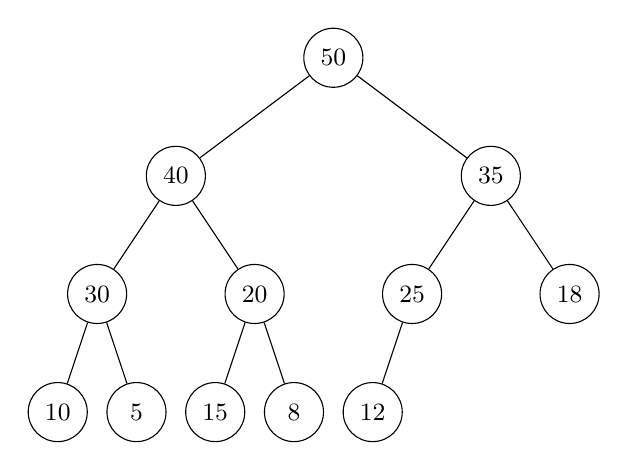
\begin{tikzpicture}[
            level distance=1.5cm, % 层与层之间的距离
            level 1/.style={sibling distance=4cm}, % 第一层节点之间的距离
            level 2/.style={sibling distance=2cm}, % 第二层节点之间的距离
            level 3/.style={sibling distance=1cm}, % 第三层节点之间的距离
            every node/.style={circle, draw, minimum size=0.75cm}, % 节点样式
            every node/.style={
                circle, % 圆形节点
                draw, % 绘制边框
                minimum size=0.75cm, % 最小大小
                inner sep=0, % 内边距为 0
                font=\small % 字体大小
            }
        ]
        
        % 绘制大根堆的二叉树结构
        \node {50} % 根节点
            child {
                node {40} % 左子节点
                child {
                    node {30} % 左子节点的左子节点
                    child { node {10} }
                    child { node {5} }
                }
                child {
                    node {20} % 左子节点的右子节点
                    child { node {15} }
                    child { node {8} }
                }
            }
            child {
                node {35} % 右子节点
                child {
                    node {25} % 右子节点的左子节点
                    child { node {12} }
                    child [missing]
                }
                child { node {18} }
            };
        \end{tikzpicture}
        \caption{A max-heap binary tree}
    \end{figure}

    \subsection{Implementation}

    \paragraph{Find Parent and Child Nodes}

    The algorithm to find the parent and child nodes of a node at index $i$ in the array representation of a binary heap is shown in Algorithm \ref{algo:Find parent and child nodes}.

    \begin{algorithm}[!htbp]
        \caption{Find parent and child nodes}
        \label{algo:Find parent and child nodes}
        \SetKwFunction{Parent}{Parent}
        \Function{\Parent{$i$}}{
            \Return{$\lfloor i/2\rfloor$}
        }

        \BlankLine

        \SetKwFunction{LeftChild}{Left-Child}
        \Function{\LeftChild{$i$}}{
            \Return{$2i$}
        }

        \BlankLine

        \SetKwFunction{RightChild}{Right-Child}
        \Function{\RightChild{$i$}}{
            \Return{$2i+1$}
        }
    \end{algorithm}

    \paragraph{Insert a New Item}

    When inserting a new item into a max-heap, we add it to the end of the array and then \highlight{float} it up to keep the max-heap property. An example to insert a new item is shown in Figure \ref{fig:Insert a new item into a max-heap binary tree}.

    \begin{figure}[!htbp]
        % 第一行:2 个子图
        \begin{minipage}{0.5\textwidth}
            \centering
            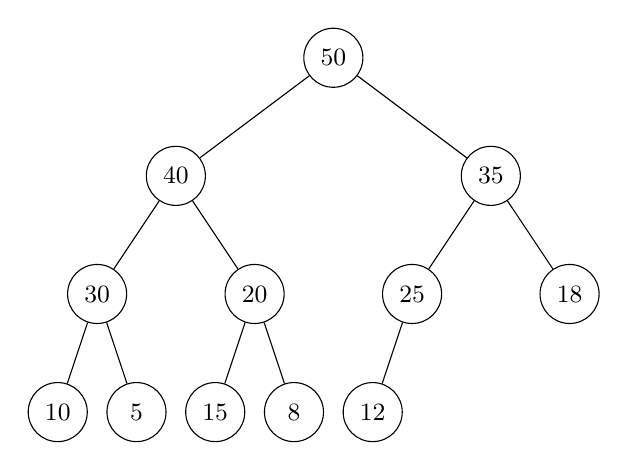
\begin{tikzpicture}[
                level distance=1.5cm,
                level 1/.style={sibling distance=4cm},
                level 2/.style={sibling distance=2cm},
                level 3/.style={sibling distance=1cm},
                every node/.style={
                    circle,
                    draw,
                    minimum size=0.75cm,
                    inner sep=0,
                    font=\small
                }
            ]
            % 初始大根堆
            \node {50}
                child {
                    node {40}
                    child {
                        node {30}
                        child { node {10} }
                        child { node {5} }
                    }
                    child {
                        node {20}
                        child { node {15} }
                        child { node {8} }
                    }
                }
                child {
                    node {35}
                    child {
                        node {25}
                        child { node {12} }
                        child[missing]
                    }
                    child { node {18} }
                };
            \end{tikzpicture}
            \subcaption{The original max-heap binary tree}
        \end{minipage}%
        \begin{minipage}{0.5\textwidth}
            \centering
            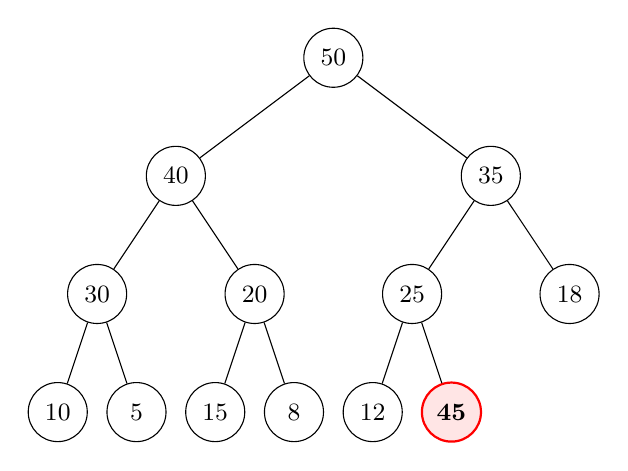
\begin{tikzpicture}[
                level distance=1.5cm,
                level 1/.style={sibling distance=4cm},
                level 2/.style={sibling distance=2cm},
                level 3/.style={sibling distance=1cm},
                every node/.style={
                    circle,
                    draw,
                    minimum size=0.75cm,
                    inner sep=0,
                    font=\small
                }
            ]
            % 初始大根堆
            \node {50}
                child {
                    node {40}
                    child {
                        node {30}
                        child { node {10} }
                        child { node {5} }
                    }
                    child {
                        node {20}
                        child { node {15} }
                        child { node {8} }
                    }
                }
                child {
                    node {35}
                    child {
                        node {25}
                        child { node {12} }
                        child { node[highlightnode] {45} }
                    }
                    child { node {18} }
                };
            \end{tikzpicture}
            \subcaption{Insert the new item 45 at the end of the array}
        \end{minipage}

        \vskip 0.5cm % 添加垂直间距
        
        % 第二行:2 个子图
        \begin{minipage}{0.5\textwidth}
            \centering
            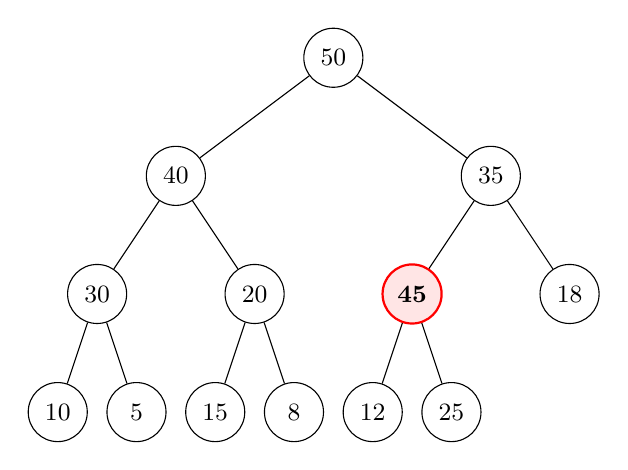
\begin{tikzpicture}[
                level distance=1.5cm,
                level 1/.style={sibling distance=4cm},
                level 2/.style={sibling distance=2cm},
                level 3/.style={sibling distance=1cm},
                every node/.style={
                    circle,
                    draw,
                    minimum size=0.75cm,
                    inner sep=0,
                    font=\small
                }
            ]
            % 初始大根堆
            \node {50}
                child {
                    node {40}
                    child {
                        node {30}
                        child { node {10} }
                        child { node {5} }
                    }
                    child {
                        node {20}
                        child { node {15} }
                        child { node {8} }
                    }
                }
                child {
                    node {35}
                    child {
                        node[highlightnode] {45}
                        child { node {12} }
                        child { node {25} }
                    }
                    child { node {18} }
                };
            \end{tikzpicture}
            \subcaption{Swap 45 with its parent 25}
        \end{minipage}%
        \begin{minipage}{0.5\textwidth}
            \centering
            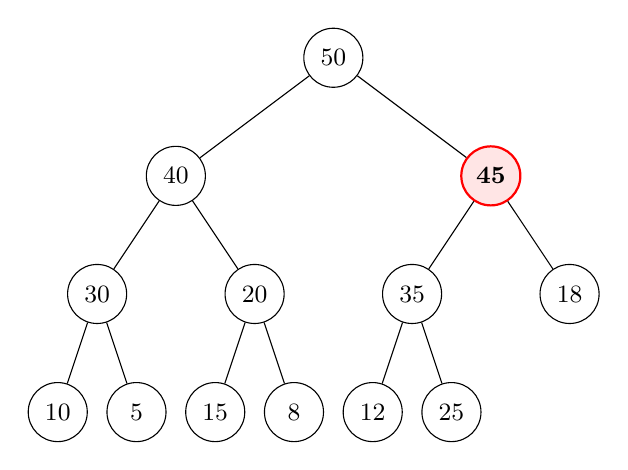
\begin{tikzpicture}[
                level distance=1.5cm,
                level 1/.style={sibling distance=4cm},
                level 2/.style={sibling distance=2cm},
                level 3/.style={sibling distance=1cm},
                every node/.style={
                    circle,
                    draw,
                    minimum size=0.75cm,
                    inner sep=0,
                    font=\small
                }
            ]
            % 初始大根堆
            \node {50}
                child {
                    node {40}
                    child {
                        node {30}
                        child { node {10} }
                        child { node {5} }
                    }
                    child {
                        node {20}
                        child { node {15} }
                        child { node {8} }
                    }
                }
                child {
                    node[highlightnode] {45}
                    child {
                        node {35}
                        child { node {12} }
                        child { node {25} }
                    }
                    child { node {18} }
                };
            \end{tikzpicture}
            \subcaption{Swap 45 with its parent 35}
        \end{minipage}
        \caption{An example of inserting a new item into a max-heap binary tree}
        \label{fig:Insert a new item into a max-heap binary tree}
    \end{figure}

    The algorithm to insert a new item into a max-heap is shown in Algorithm \ref{algo:Add a new item to a max-heap}.

    \begin{algorithm}[!htbp]
        \caption{Add a new item to a max-heap}
        \label{algo:Add a new item to a max-heap}
        \SetKwFunction{Insert}{Insert}
        \SetKwFunction{FloatUp}{Float-Up}
        \Function{\Insert{$A,x$}}{
            \SetKwFunction{Pushback}{Push-back}
            $A.\Pushback(x)$\;
            $A.\textit{size} \gets A.\textit{size} + 1$\;
            \FloatUp{$A.\textit{size}$}\;
        }
        \BlankLine
        \Function{\FloatUp{$i$}}{
            \While{$i > 1$ and $A[i] > A[\Parent{i}]$}{
                Swap $A[i]$ and $A[\Parent{i}]$\;
                $i \gets \Parent{i}$\;
            }
        }
    \end{algorithm}

    \subsection{Delete the Highest-Priority Item}

    When deleting the highest-priority item from a max-heap, we first swap the root with the last item in the array, then \highlight{sink} the new root down to keep the max-heap property. An example to delete the highest-priority item is shown in Figure \ref{fig:Delete the highest-priority item from a max-heap binary tree}.

    \begin{figure}[!htbp]
        % 第一行:2 个子图
        \begin{minipage}{0.5\textwidth}
            \centering
            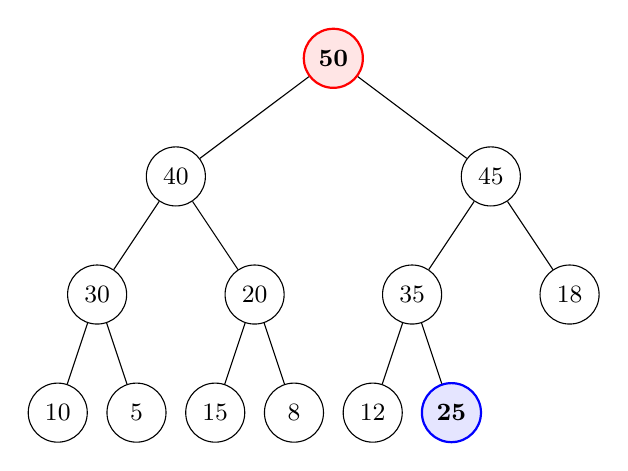
\begin{tikzpicture}[
                level distance=1.5cm,
                level 1/.style={sibling distance=4cm},
                level 2/.style={sibling distance=2cm},
                level 3/.style={sibling distance=1cm},
                every node/.style={
                    circle,
                    draw,
                    minimum size=0.75cm,
                    inner sep=0,
                    font=\small
                }
            ]
            % 初始大根堆
            \node[highlightnode] {50}
                child {
                    node {40}
                    child {
                        node {30}
                        child { node {10} }
                        child { node {5} }
                    }
                    child {
                        node {20}
                        child { node {15} }
                        child { node {8} }
                    }
                }
                child {
                    node {45}
                    child {
                        node {35}
                        child { node {12} }
                        child { node[bluenode] {25} }
                    }
                    child { node {18} }
                };
            \end{tikzpicture}
            \subcaption{The original max-heap binary tree}
        \end{minipage}%
        \begin{minipage}{0.5\textwidth}
            \centering
            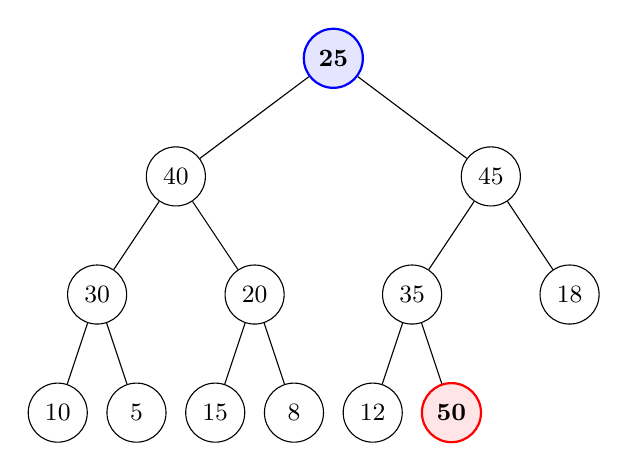
\begin{tikzpicture}[
                level distance=1.5cm,
                level 1/.style={sibling distance=4cm},
                level 2/.style={sibling distance=2cm},
                level 3/.style={sibling distance=1cm},
                every node/.style={
                    circle,
                    draw,
                    minimum size=0.75cm,
                    inner sep=0,
                    font=\small
                }
            ]
            % 初始大根堆
            \node[bluenode] {25}
                child {
                    node {40}
                    child {
                        node {30}
                        child { node {10} }
                        child { node {5} }
                    }
                    child {
                        node {20}
                        child { node {15} }
                        child { node {8} }
                    }
                }
                child {
                    node {45}
                    child {
                        node {35}
                        child { node {12} }
                        child { node[highlightnode] {50} }
                    }
                    child { node {18} }
                };
            \end{tikzpicture}
            \subcaption{Swap the root with the last item in the array}
        \end{minipage}

        \vskip 0.5cm % 添加垂直间距

        % 第二行:2 个子图
        \begin{minipage}{0.5\textwidth}
            \centering
            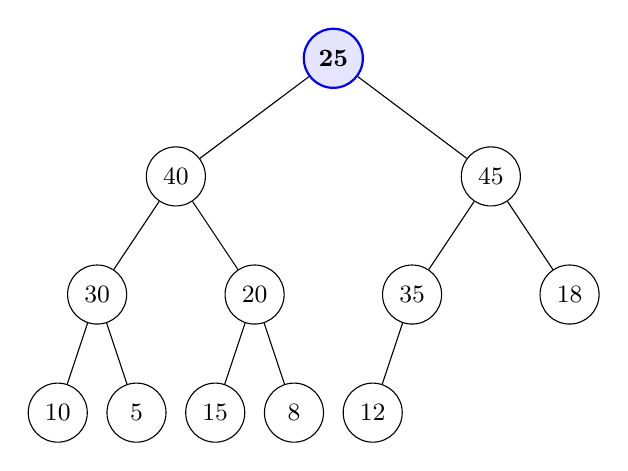
\begin{tikzpicture}[
                level distance=1.5cm,
                level 1/.style={sibling distance=4cm},
                level 2/.style={sibling distance=2cm},
                level 3/.style={sibling distance=1cm},
                every node/.style={
                    circle,
                    draw,
                    minimum size=0.75cm,
                    inner sep=0,
                    font=\small
                }
            ]
            % 初始大根堆
            \node[bluenode] {25}
                child {
                    node {40}
                    child {
                        node {30}
                        child { node {10} }
                        child { node {5} }
                    }
                    child {
                        node {20}
                        child { node {15} }
                        child { node {8} }
                    }
                }
                child {
                    node {45}
                    child {
                        node {35}
                        child { node {12} }
                        child[missing]
                    }
                    child { node {18} }
                };
            \end{tikzpicture}
            \subcaption{Delete the last item in the array}
        \end{minipage}%
        \begin{minipage}{0.5\textwidth}
            \centering
            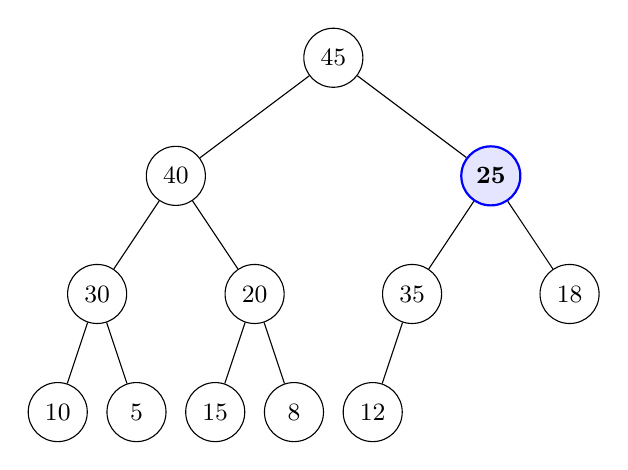
\begin{tikzpicture}[
                level distance=1.5cm,
                level 1/.style={sibling distance=4cm},
                level 2/.style={sibling distance=2cm},
                level 3/.style={sibling distance=1cm},
                every node/.style={
                    circle,
                    draw,
                    minimum size=0.75cm,
                    inner sep=0,
                    font=\small
                }
            ]
            \node {45}
                child {
                    node {40}
                    child {
                        node {30}
                        child { node {10} }
                        child { node {5} }
                    }
                    child {
                        node {20}
                        child { node {15} }
                        child { node {8} }
                    }
                }
                child {
                    node[bluenode] {25}
                    child {
                        node {35}
                        child { node {12} }
                        child [missing]
                    }
                    child { node {18} }
                };
            \end{tikzpicture}
            \subcaption{Swap the new root with its largest child 45}
        \end{minipage}
        
        \vskip 0.5cm % 添加垂直间距

        \begin{minipage}{0.5\textwidth}
            \centering
            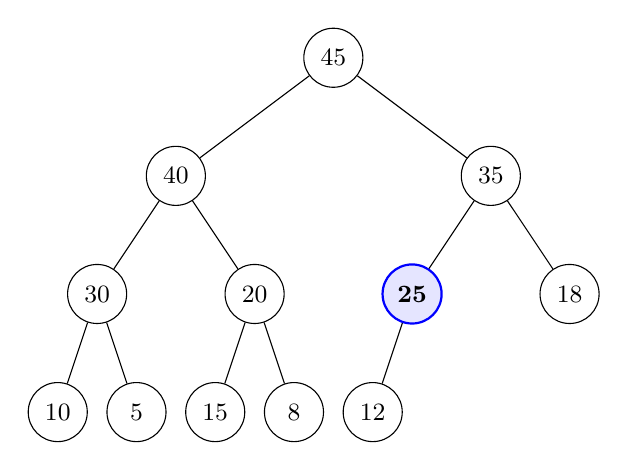
\begin{tikzpicture}[
                level distance=1.5cm,
                level 1/.style={sibling distance=4cm},
                level 2/.style={sibling distance=2cm},
                level 3/.style={sibling distance=1cm},
                every node/.style={
                    circle,
                    draw,
                    minimum size=0.75cm,
                    inner sep=0,
                    font=\small
                }
            ]
            \node {45}
                child {
                    node {40}
                    child {
                        node {30}
                        child { node {10} }
                        child { node {5} }
                    }
                    child {
                        node {20}
                        child { node {15} }
                        child { node {8} }
                    }
                }
                child {
                    node {35}
                    child {
                        node[bluenode] {25}
                        child { node {12} }
                        child [missing]
                    }
                    child { node {18} }
                };
            \end{tikzpicture}
            \subcaption{Swap 25 with its largest child 35}
        \end{minipage}
        
        \caption{An example of deleting the highest-priority item from a max-heap binary tree}
        \label{fig:Delete the highest-priority item from a max-heap binary tree}
    \end{figure}
\end{document}